\chapter{Аналитическая часть}

В данном разделе описана структура рабочей программы дисциплины. Представлен анализ способов хранения данных и систем управления базами данных, оптимальных для решения поставленной задачи. Описаны проблемы кэшированных данных и представлены методы их решения.

\section{Формализация задачи}

Каждая дисциплина, преподаваемая в высшем учебном заведении, имеет свою рабочую программу. В ней хранятся различная информация о дисциплине: стандарт, содержание, объем, результаты обучения, перечень литературы, методические указания и прочее. Зачастую, у пользователей нет никаких автоматизированных инструментов для анализа и редактирования таких программ.

Дисциплина имеет свой федеральный государственный образовательный стандарт: 3+, 3++ и другие \cite{standard}. Образовательный стандарт -- это совокупность обязательных требований к образованию определенного уровня и (или) к профессии, специальности. Каждый образовательный стандарт для каждого направления подготовки обучаемого имеет свою компетенцию. Компетенция -- некоторый свод информации, о том что должен знать, уметь и какими навыками должен обладать выпускник, успешно осовевший дисциплину. 

Каждому направлению подготовки, но одной и той же рабочей программы дисциплины сопоставлены различные компетенции (которые, в свою очередь, различны в каждом образовательном стандарте). Например, есть два студента, успешно осовевшие дисциплину <<Физика>>. Один из них обучается по направлению подготовки <<Экономика>>, а второй по направлению <<Теплофизика и теоретическая теплотехника>>. Очевидно, что второй студент должен владеть большими знаниями о данной дисциплине.

Коды компетенций для каждого образовательного стандарта отличаются. К сожалению, не редки случаи, когда при переходе на новую образовательную программу меняется только код и название компетенции -- содержание компетенции остается абсолютно точно таким же. В связи с этим, возникает возможность автоматизации перевода документов рабочей программы дисциплины на новый стандарт.

Кроме того, имея данные о всех рабочих программах дисциплинах, можно адаптировать какие-либо из них под выбранные направления подготовки. Например, рассчитать оптимальную нагрузку по данной дисциплине для студентов обучающихся на данном направлении.

Далее, в качестве примера, будем рассматривать рабочую программу дисциплины <<Информатика>>, соответствующую образовательному стандарту 3++, разработанную и преподаваемую в МГТУ им. Н. Э. Баумана \cite{bmstu}.

\section{Структура рабочей программы дисциплины} \label{sec:rpd-structure}

Структура файлов рабочих программ дисциплин можно разниться от ВУЗа к ВУЗу, но, внутри одного ВУЗа, скорее всего, все программы имеют одну и ту же (или схожую) структуру. Рабочая программа дисциплины <<Информатика>> имеет следующие разделы:

\begin{enumerate}
	\item титульный лист;
	\item планируемые результаты обучения по дисциплине, соотнесенные с планируемыми результатами освоения образовательной программы;
	\item место дисциплины в структуре образовательной программы;
	\item объем дисциплины;
	\item содержание дисциплины;
	\item учебно-методическое обеспечение самостоятельно работы;
	\item фонд оценочных средств для проведения текущего контроля и промежуточной аттестации студентов;
	\item перечень основной и дополнительной литературы;
	\item методические указания;
	\item перечень информационных технологий;
	\item описание материально-технической базы.
\end{enumerate}

Разделы №2, №4, №5 представленны в виде совокупности текстовой информации и таблиц (рис. \ref{img:rpd_example_01}). Остальные разделы представлены в виде текстовой информации (рис. \ref{img:rpd_example_02}).

\begin{figure}[h!]
	\begin{center}
		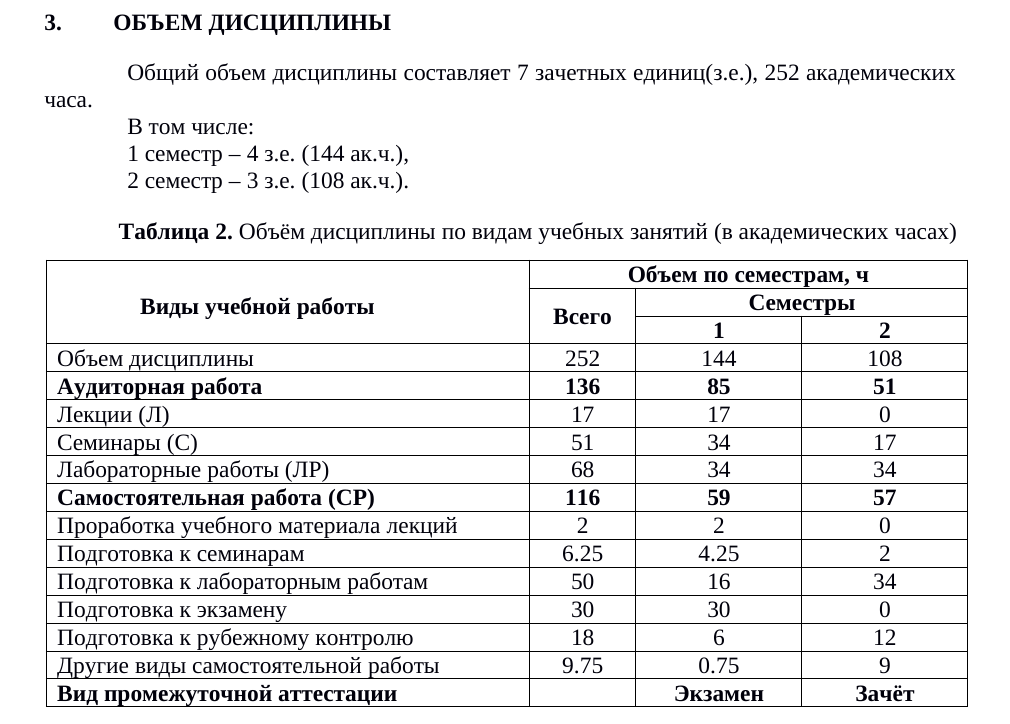
\includegraphics[scale=0.5]{img/rpd_example_02.png}
	\end{center}
	\captionsetup{justification=centering}
	\caption{Изображение таблицы c информацией о объеме дисциплины.}
	\label{img:rpd_example_01}
\end{figure}

\begin{figure}[h!]
	\begin{center}
		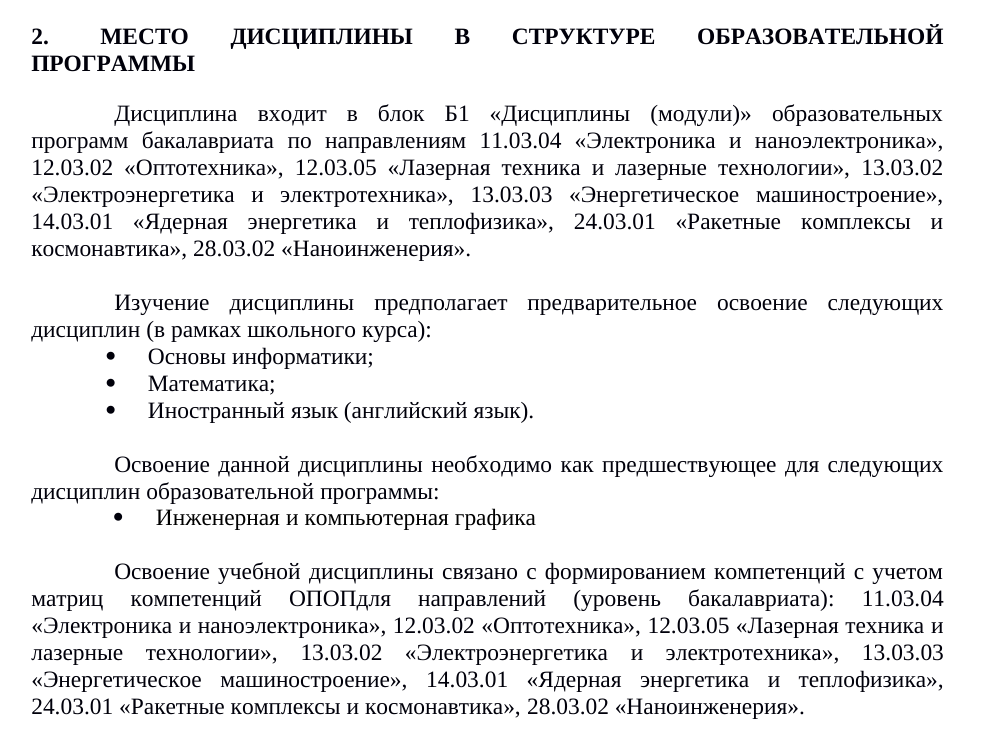
\includegraphics[scale=0.5]{img/rpd_example_01.png}
	\end{center}
	\captionsetup{justification=centering}
	\caption{Изображение текстовой информации о месте дисциплине в структуре образовательной программы.}
	\label{img:rpd_example_02}
\end{figure}

Интерес представляют разделы №1 (титульный лист), №2 (результаты обучения), №4 (объем дисциплины), №5 (содержание дисциплины) и №8 (перечень литературы). 

Первый раздел содержит общую информацию о курсе: название, образовательный стандарт и прочее. 

Раздел №2 содержит коды и описания компетенций для каждого направления подготовки. С помощью информации, полученной в этом разделе, можно попробовать автоматизировать перенос файла рабочей программы дисциплины с одной образовательной программы на другую.

В разделах №4 и №5 хранится информация о нагрузке и структуре дисциплины -- эта информация может пригодится для анализа нагрузки на студентов по выбранному направлению подготовки и структуризации рассматриваемой рабочей программы дисциплины.

\section{Базы данных и системы управления базами данных}

В задаче разбора и хранения информации рабочей программы дисциплины важную роль имеет выбор модели хранения данных. Для персистентного хранения данных используются базы данных \cite{database}. Для управления этими базами данных используется системы управления данных -- СУБД \cite{subd}. Система управления базами данных -- это совокупность программных и лингвистических средств общего или специального назначения, обеспечивающих управление созданием и использованием баз данных.

\section{Хранение данных о рабочих программах дисциплины}

Система, разрабатываемая в рамках курсового проекта, предполагает собой приложение, которое является микросервисом \cite{microservice} одной большой системы -- системы управления обучения. 

Предполагается, что доступ к разрабатываемому приложению будем иметь лишь только <<ядро>> этой системы. При этом, только у одного типа пользователя системы есть доступ к данным, хранящимся в приложении -- преподавателю. Состояние гонки (англ. Race condition \cite{race-condition}) можно исключить - каждый преподаватель работает только с информацией из файлов, которые он самостоятельно загрузил в базу данных.

Для хранения данных о рабочей программы дисциплины необходимо использовать строго структурированную и типизированную базу данных, потому что вся информация, предоставленная в файлах программы имеет чётко выраженную структуру, которая не будет меняться от дисциплины к дисциплине.

\subsection{Классификация баз данных по способу хранения}

Базы данных, по способу хранения, делятся на две группы -- строковые и колоночные. Каждый из этих типов служит для выполнения для определенного рода задач.

\noindent\textbf{Строковые базы данных}\\

Строковыми базами даных называются такие базы данных, записи которых в памяти представляются построчно. Строковые баз данных используются в транзакционных системах (англ. OLTP \cite{OLTP}). Для таких систем характерно большое количество коротких транзакций с операциями вставки, обновления и удаления данных - \texttt{INSERT}, \texttt{UPDATE}, \texttt{DELETE}. 

Основной упор в системах OLTP делается на очень быструю обработку запросов, поддержание целостности данных в средах с множественным доступом и эффективность, которая измеряется количеством транзакций в секунду. 

Схемой, используемой для хранения транзакционных баз данных, является модель сущностей, которая включает в себя запросы, обращающиеся к отдельным записям. Так же, в OLTP-системах есть подробные и текущие данных.\\

\noindent\textbf{Колоночные базы данных}\\

Колоночными базами данных называются базы данных, записи которых в памяти представляются по столбцам. Колоночные базы данных используется в аналитических системах (англ. OLAP \cite{olap}). OLAP характеризуется низким объемом транзакций, а запросы часто сложны и включают в себя агрегацию. Время отклика для таких систем является мерой эффективности.

OLAP-системы широко используются методами интеллектуального анализа данных. В таких базах есть агрегированные, исторические данные, хранящиеся в многомерных схемах. 

\subsection{Выбор модели хранения данных для решения задачи}

Для решения задачи построчное хранение данных преобладает над колоночным хранением по нескольким причинам:

\begin{itemize}
	\item задача предполагает постоянное добавление и изменение данных;
	\item задача предполагает быструю отзывчивость на запросы пользователя;
	\item задача не предполагает выполнения аналитических запросов;
\end{itemize}

\subsection{Обзор СУБД с построчным хранение}

В данном подразделе буду рассмотрены популярные построчные СУБД, которые могут быть использованы для реализации хранения в разрабатываемом программном продукте.\\

\noindent\textbf{PostgreSQL}\\

PostgreSQL \cite{postgresql} -- это свободно распространяемая объектно-реляционная система управления базами данных, наиболее развитая из открытых СУБД в мире и являющаяся реальной альтернативой коммерческим базам данных \cite{postgresql-fact}.

PostgreSQL предоставляет транзакции со свойствами атомарности, согласованности, изоляции, долговечности (ACID \cite{acid}), автоматически обновляемые представления, материализованные представления, триггеры, внешние ключи и хранимые процедуры. Данная СУБД предназначена для обработки ряда рабочих нагрузок, от отдельных компьютеров до хранилищ данных или веб-сервисов с множеством одновременных пользователей. 

Рассматриваемая СУБД управляет параллелизмом с помощью технологии управления многоверсионным параллелизмом (англ. MVCC \cite{mvcc}). Эта технология дает каждой транзакции <<снимок>> текущего состояния базы данных, позволяя вносить изменения, не затрагивая другие транзакции. Это в значительной степени устраняет необходимость в блокировках чтения (англ. read lock \cite{r-lock}) и гарантирует, что база данных поддерживает принципы ACID. \\

\noindent\textbf{Oracle Database}\\

Oracle Database \cite{oracle} -- объектно-реляционная система управления базами данных компании Oracle \cite{oracle-company}. На данный момент, рассматриваемая СУБД является самой популярной в мире. \cite{oracle-popular}

Все транзакции Oracle Database соответствуют обладают свойствами ACID, поддерживает триггеры, внешние ключи и хранимые процедуры. Данная СУБД подходит для разнообразных рабочих нагрузок и может использоваться практически в любых задачах. Особенностью Oracle Database является быстрая работа с большими массивами данных.

Oracle Database может использовать один или более методов параллелизма. Сюда входят механизмы блокировки для гарантии монопольного использования таблицы одной транзакцией, методы временных меток, которые разрешают сериализацию транзакций и планирование транзакций на основе проверки достоверности. \\

\noindent\textbf{MySQL}\\

MySQL \cite{mysql} -- свободная реляционная система управления базами данных. Разработку и поддержку MySQL осуществляет корпорация Oracle.

Рассматриваемая СУБД имеет два основных движка хранения данных: InnoDB \cite{innodb} и myISAM \cite{myisam}. Движок InnoDB полностью полностью совместим с принципами ACID, в отличии от движка myISAM. СУБД MySQL подходит  для использования при разработке веб-приложений, что объясняется очень тесной интеграцией с популярными языками PHP \cite{php} и Perl \cite{perl}.

Реализация параллелизма в СУБД MySQL реализовано с помощью механизма блокировок, который обеспечивает одновременный доступ к данным.

\subsection{Выбор СУБД для решения задачи}

Для решения задачи была выбрана СУБД PostgreSQL, потому что данная СУБД имеет поддержку языка plpython3u \cite{plpython3u}, который упрощает процесс интеграции базы данных в разрабатываемое приложение. Кроме того, PostgreSQL проста в развертывании.

\section{Кэширование данных}

Для ускорения быстродействия разрабатываемого приложения, можно прибегнуть к кэшированию данных. Для кэширования данных можно  использовать NoSQL \cite{nosql} in-memory базы данных. Такие базы данных хранят данные в оперативной памяти, что обеспечивает более быстрый доступ к данным.

\subsection{Проблемы кэширования данных}

\noindent\textbf{Синхронизация данных}\\

Приложение пишет в кэш, и в базу данных, которые между собой никак не синхронизируются. Таким образом возникает несогласованность данных. Например, в случае разрабатываемого приложения, возможна ситуация, когда данные удаляются из хранилища и их нужно удалить из
кэша. Эту проблему можно решить установкой триггеров в базе данных хранения рабочих программ дисциплин, которые буду срабатывать на изменение / удаление данных и синхронизировать актуальные данные в кэше.\\

\noindent\textbf{Проблема <<холодного старта>>}\\

Когда кэш только развертывается, он пуст и в нем нет никаких данных. Все запросы идут напрямую в базу данных, и только спустя какое-то время кэш будет <<разогрет>> и будет работать в полную силу. Эту проблему можно решить, выбрав СУБД с журналированием всех операций: при перезагрузке можно восстановить предыдущее состояние кэша с помощью журнала событий, который хранится на диске. При этом, при перезапуске кэша, нужно синхронизировать данные с хранилищем: возможно, какие-то данные находящиеся в кэше перестали быть актуальными за время его перезагрузки.

\subsection{Обзор in-memory NoSQL СУБД}

\noindent\textbf{Tarantool}\\

Tarantool \cite{tarantool} -- это платформа in-memory вычислений с гибкой схемой хранения данных для эффективного создания высоконагруженных приложений. Включает себя базу данных и сервер приложений на языке программирования Lua \cite{lua}.

Tarantool обладает высокой скоростью работы по сравнению с традиционными СУЬД.  При этом, в рассматриваемой платформе для транзакций реализованы свойства ACID, репликация master-slave \cite{master-slave} и master-master \cite{master-master}, как и в традиционных СУБД.

Для хранения данных используется кортежи (англ. tuple) данных. Кортеж -- это массив не типизированных данных. Кортежи объединяются в спейсы (англ. space), аналоги таблицы из реляционной модели хранения данных. Спейс -- коллекция кортежей, кортеж -- коллекция полей.

В рассматриваемой СУБД реализованы два движка хранения данных: memtx \cite{memtx-vinyl} и vinyl \cite{memtx-vinyl}. Первый хранит все данные в оперативной памяти, а второй на диске. Для каждого спейса можно задавать различный движок хранения данных. 

Каждый спейс должен быть проиндексирован первичным ключом. Кроме того, поддерживается неограниченное количество вторичных ключей. Каждый из ключей может быть составным.

В Tarantool реализован механизм <<снимков>> текущего состояния хранилища и журналирования всех операций, что позволяет восстановить состояние базы данных после ее перезагрузки.\\

\noindent\textbf{Redis}\\

Redis \cite{redis} -- резидентная система управлениями базами данных класса NoSQL с открытым исходным кодом. Основной структурой данных, с которой работает Redis является структура типа <<ключ-значение>>. Данная СУБД используется как для хранения данных, так и для реализации кэшей и брокеров сообщений.

Redis хранит данные в оперативной памяти и снабжена механизмом <<снимков>> и журналирования, что обеспечивает постоянное хранение данных. Предоставляются операции для реализации механизма обмена сообщениями в шаблоне <<издатель-подписчик>>: с его помощью приложения могут создавать программные каналы, подписываться на них и помещать в эти каналы сообщения, которые будут получены всеми подписчиками. Существует поддержка репликации данных типа master-slave, транзакций и пакетной обработки комманд.

Все данные Redis хранит в виде словаря, в котором ключи связаны со своими значениями. Ключевое отличие Redis от других хранилищ данных заключается в том, что значения этих ключей не ограничиваются строками. Поддерживаются следующие абстрактные типы данных:

\begin{itemize}
	\item строки;
	\item списки;
	\item множества;
	\item хеш-таблицы;
	\item упорядоченные множества.
\end{itemize}

Тип данных значения определяет, какие операции доступные для него; поддежриваются высокоуровневые операции: например, объединение, разность или сортировка наборов.

\subsection{Выбор СУБД для решения задачи}

Для кэширования данных была выбрана СУБД Tarantool, так как она проста в развертывании и переносимости, и имеет подходящие коннекторы для базы данных PostgreSQL.

\section{Формализация данных}

\subsection{База данных рабочих программ дисциплин}

База данных рабочих программ дисциплин должна хранить непосредственно информацию о дисциплинах. Информация, которая должна хранится в базе данных описана в разделе \ref{sec:rpd-structure}. Каждая рабочая дисциплина должна обладать уникальным идентификатором, чтобы её можно было однозначно идентифицировать.

\subsection{База данных кэшируемой информации}

База данных кэшируемых значений должна хранить значения без дополнительной обработки. Данные должны быть актуальны и синхронизированны с основным хранилищем: кэш должен обновляться после каждой транзакции. Кроме того, нужно ограничить размер кэша и добавить вытеснение из него, например, с помощью политики вытеснения LRU \cite{lru} (Last Recently Used).

\section*{Вывод}

В данном разделе:

\begin{itemize}
 \item рассмотрена структура рабочей программы дисциплины и выявлены её наиболее интересные части;
 \item проанализированы способы хранения информации для система и выбраны оптимальные способы для решения поставленной задачи; 
 \item проведен анализ СУБД, используемых для решения задачи и также выбраны оптимальные информационные системы; 
 \item рассмотрена проблема актуальности кэшируемых данных и предложенно ее решение;
 \item формализованны данные, используемые в системе.
\end{itemize}

